% =====================================================================
%  Trabalho da Unidade 1 - IMD0039 Estruturas de Dados Basicas II
%  Analise Empirica de Algoritmos
%
%  Compilacao:  pdflatex main.tex  (duas vezes, por causa das referencias)
%  Depende de:  resultados/tabelas.tex   (gerado por codigo/gerar_graficos.py)
%               figuras/*.pdf            (gerado por codigo/gerar_graficos.py)
% =====================================================================
\documentclass[12pt,a4paper]{article}

\usepackage[utf8]{inputenc}
\usepackage[T1]{fontenc}
\usepackage[brazil]{babel}
\usepackage[margin=2.5cm]{geometry}
\usepackage{graphicx}
\usepackage{booktabs}
\usepackage{multirow}
\usepackage{amsmath,amssymb}
\usepackage{listings}
\usepackage{xcolor}
\usepackage[font=small,labelfont=bf]{caption}
\usepackage{float}
\usepackage{algorithm}
\usepackage{algpseudocode}
\usepackage[hidelinks]{hyperref}
\usepackage{setspace}

% ----- macro para marcar o que o grupo ainda precisa preencher --------
\newcommand{\pendente}[1]{\textcolor{red}{\textbf{[PREENCHER: #1]}}}

% ----- estilo dos trechos de codigo ----------------------------------
\definecolor{cinzafundo}{RGB}{247,247,247}
\definecolor{verdecom}{RGB}{0,110,60}
\definecolor{azulkw}{RGB}{20,60,150}
\lstdefinestyle{cpp}{
  language=C++, basicstyle=\ttfamily\scriptsize, backgroundcolor=\color{cinzafundo},
  keywordstyle=\color{azulkw}\bfseries, commentstyle=\color{verdecom}\itshape,
  numbers=left, numberstyle=\tiny\color{gray}, numbersep=7pt,
  breaklines=true, frame=single, framerule=0.3pt, rulecolor=\color{gray},
  showstringspaces=false, tabsize=2, captionpos=b, aboveskip=8pt, belowskip=8pt,
  literate={á}{{\'a}}1 {é}{{\'e}}1 {í}{{\'i}}1 {ó}{{\'o}}1 {ú}{{\'u}}1
           {ã}{{\~a}}1 {õ}{{\~o}}1 {ç}{{\c c}}1 {ê}{{\^e}}1 {â}{{\^a}}1
}
\lstset{style=cpp}

\algrenewcommand\algorithmicrequire{\textbf{Entrada:}}
\algrenewcommand\algorithmicensure{\textbf{Saída:}}
\floatname{algorithm}{Algoritmo}
\renewcommand{\listalgorithmname}{Lista de Algoritmos}

% ----- dados numericos gerados automaticamente pelo experimento ------
% Arquivo gerado automaticamente por codigo/gerar_graficos.py
% Nao editar a mao: reexecute o script apos novas medicoes.
\newcommand{\numRepeticoes}{5}
\newcommand{\desvioRelMax}{12.6}
\newcommand{\desvioRelMaior}{10.4}
\newcommand{\linhasMedias}{%
1.000 & 4.000 & 0.729 & 0.078 & 0.160 & 0.020 & 0.111 & 0.014 \\
2.000 & 8.000 & 2.632 & 0.131 & 0.317 & 0.012 & 0.189 & 0.014 \\
4.000 & 16.000 & 9.973 & 0.135 & 0.715 & 0.014 & 0.325 & 0.007 \\
8.000 & 32.000 & 40.452 & 0.736 & 1.621 & 0.147 & 0.609 & 0.034 \\
16.000 & 64.000 & 182.890 & 1.498 & 3.594 & 0.104 & 1.112 & 0.024 \\
32.000 & 128.000 & 1479.760 & 9.486 & 8.317 & 0.160 & 2.243 & 0.069 \\
64.000 & 256.000 & 6897.924 & 7.108 & 19.921 & 0.938 & 5.386 & 0.559 \\}
\newcommand{\linhasRazoes}{%
1.000 $\rightarrow$ 2.000 & 3.61 & 1.98 & 1.70 \\
2.000 $\rightarrow$ 4.000 & 3.79 & 2.26 & 1.72 \\
4.000 $\rightarrow$ 8.000 & 4.06 & 2.27 & 1.87 \\
8.000 $\rightarrow$ 16.000 & 4.52 & 2.22 & 1.83 \\
16.000 $\rightarrow$ 32.000 & 8.09 & 2.31 & 2.02 \\
32.000 $\rightarrow$ 64.000 & 4.66 & 2.40 & 2.40 \\}
\newcommand{\linhasConstantes}{%
1.000 & 0.729 & 16.06 & 110.8 \\
2.000 & 0.658 & 14.43 & 94.3 \\
4.000 & 0.623 & 14.94 & 81.3 \\
8.000 & 0.632 & 15.63 & 76.2 \\
16.000 & 0.714 & 16.08 & 69.5 \\
32.000 & 1.445 & 17.37 & 70.1 \\
64.000 & 1.684 & 19.50 & 84.2 \\}
\newcommand{\linhasEstruturais}{%
1.000 & 1.737 & 1.938 & 9 \\
2.000 & 1.930 & 1.991 & 18 \\
4.000 & 2.167 & 2.167 & 35 \\
8.000 & 2.232 & 2.246 & 70 \\
16.000 & 2.229 & 2.229 & 141 \\
32.000 & 2.593 & 2.593 & 281 \\
64.000 & 2.615 & 2.615 & 562 \\}
\newcommand{\expoenteNormal}{2.22}
\newcommand{\expoenteHeap}{1.17}
\newcommand{\expoenteBucket}{0.92}
\newcommand{\ganhoHeap}{346}
\newcommand{\ganhoBucket}{1281}
\newcommand{\heapSobreBucket}{3.7}
\newcommand{\nMin}{1.000}
\newcommand{\nMax}{64.000}
\newcommand{\tempoMaxNormal}{6898}
\newcommand{\tempoMaxHeap}{19.9}
\newcommand{\tempoMaxBucket}{5.4}


% =====================================================================
\begin{document}

% ----------------------------------------------------------- capa
\begin{titlepage}
\centering
\vspace*{1cm}

{\large UNIVERSIDADE FEDERAL DO RIO GRANDE DO NORTE\par}
{\large INSTITUTO METRÓPOLE DIGITAL\par}
\vspace{0.3cm}
{\large IMD0039 --- Estruturas de Dados Básicas II\par}

\vfill

{\Huge\bfseries Análise Empírica de Algoritmos\par}
\vspace{0.6cm}
{\LARGE O impacto da estrutura de dados da fila de prioridade\\ no tempo de execução do algoritmo de Dijkstra\par}

\vspace{1.2cm}
{\large Trabalho da Unidade 1\par}

\vfill

{\large\bfseries Integrantes do grupo\par}
\vspace{0.3cm}
\begin{tabular}{ll}
Luiz Carlos Victor Pinto & 20250024456 \\
Marcus Vinicius de Lima Souza & 20250032716 \\
Eduardo Queiroz Cavalcanti Gomes & 20250033947 \\
Davi Summer Silva Costa & 20250033590 \\
\end{tabular}

\vspace{1.2cm}
{\large Profa. Ligia Borges\par}

\vfill
{\large Currais Novos / Natal --- RN\par}
{\large \today\par}
\end{titlepage}

\onehalfspacing
\pagenumbering{roman}
\tableofcontents
\newpage
\pagenumbering{arabic}

% =====================================================================
\section{Introdução}
% =====================================================================

O problema do caminho mínimo consiste em determinar, em um grafo com pesos
não negativos nas arestas, o menor custo para ir de um vértice de origem até
todos os demais vértices. É um dos problemas mais aplicados da computação:
aparece em sistemas de navegação, em roteamento de pacotes em redes, em
planejamento logístico e em problemas de otimização em geral. O algoritmo
clássico para resolvê-lo é o algoritmo de Dijkstra, publicado em 1959
(DIJKSTRA, 1959).

O ponto que motiva este trabalho é que o algoritmo de Dijkstra não é um único
algoritmo, e sim um \emph{esqueleto}: ele repete o par de operações
``extrair o vértice aberto de menor distância estimada'' e ``relaxar as
arestas desse vértice'' até fechar todos os vértices. A ordem em que os
vértices são visitados e o resultado final são sempre os mesmos, mas o
\textbf{custo} da operação de extração do mínimo depende inteiramente da
estrutura de dados usada para manter a fila de prioridade. Isso faz do
Dijkstra um caso quase ideal para uma investigação empírica: é possível
manter fixos o problema, a entrada, a linguagem e o compilador, e variar
apenas a estrutura de dados.

Este relatório investiga, portanto, a seguinte pergunta:

\begin{quote}
\itshape Como o tempo de execução do algoritmo de Dijkstra cresce em função
do número de vértices do grafo, e de que forma esse crescimento muda quando
a fila de prioridade é implementada por varredura linear de vetor, por
\emph{heap} mínimo e por \emph{buckets}?
\end{quote}

Foram implementadas e medidas três variantes: o \textbf{Dijkstra Normal}
(seleção do mínimo por varredura linear, $O(n^2)$), o \textbf{Dijkstra com
Heap Mínimo} (fila de prioridade em \emph{heap} binário, $O((n+m)\log n)$) e
o \textbf{Dijkstra com Buckets}, na formulação de Dial (fila de prioridade
monótona com \emph{buckets} circulares, $O(m + n + D_{max})$). O objetivo do
experimento é verificar se o crescimento observado é compatível com essas
previsões assintóticas e, onde houver divergência, identificar a causa.

% =====================================================================
\section{Algoritmos e fontes}
% =====================================================================

\subsection{Como as fontes foram localizadas}

A busca partiu do tema ``caminho mínimo em grafos'' com foco em trabalhos que
comparassem estruturas de dados de forma experimental.

\begin{itemize}
  \item \textbf{Palavras-chave utilizadas:} "algoritmo", "djikstra", "desempenho"
  \item \textbf{Base/local de busca:} Google Acadêmico
  \item \textbf{Data de acesso:} 07/09/2026
\end{itemize}

\subsection{Fonte principal}

\begin{quote}
RODRIGUES, Guilherme Conrado da Silva. \textbf{Análise de desempenho do
algoritmo de Dijkstra com diferentes estruturas de dados}. 2023. Trabalho de
Conclusão de Curso (Bacharelado em Ciência da Computação) --- Departamento de
Computação, Centro de Ciências Exatas, Naturais e da Saúde, Universidade
Federal do Espírito Santo, Alegre, ES, 2023. Orientador: Prof. Dr. Edmar Hell
Kampke. Aprovado em 15 de dezembro de 2023.
\end{quote}

\noindent
\textbf{Repositório de código indicado pela fonte:}
\url{https://github.com/guiconrado/Djkstra}

Esse TCC foi escolhido como fonte principal por três razões: (i) apresenta os
pseudocódigos completos das três variantes que queríamos comparar; (ii) informa
explicitamente a complexidade esperada de cada uma; e (iii) já executa uma
comparação de desempenho, o que nos dá um resultado de referência contra o
qual confrontar as nossas medições.

O trabalho de referência mediu as três variantes sobre quatro instâncias reais
de redes de estradas dos Estados Unidos, obtidas do \emph{9th DIMACS
Implementation Challenge --- Shortest Paths}, e obteve tempos médios de
$407{,}242$~s para o Dijkstra Normal, $0{,}032$~s para o Heap Mínimo e
$0{,}184$~s para o Bucket, concluindo que o Heap Mínimo foi cerca de seis vezes
mais rápido que o Bucket naquele conjunto de testes.

\subsection{Algoritmos selecionados}

\begin{table}[H]
\centering
\caption{Algoritmos comparados neste trabalho.}
\label{tab:algoritmos}
\small
\begin{tabular}{@{}p{2.6cm}p{3.4cm}p{3.2cm}p{4.4cm}@{}}
\toprule
\textbf{Algoritmo} & \textbf{Estrutura da fila de prioridade} &
\textbf{Complexidade indicada pela fonte} & \textbf{Contexto de aplicação} \\
\midrule
Dijkstra Normal & Vetor de distâncias com varredura linear &
$O(n^2)$ &
Grafos densos ou pequenos; implementação de referência, usada em ensino \\
\addlinespace
Dijkstra Heap Mínimo & \emph{Heap} binário (fila de prioridade) &
$O((n+m)\log n)$ &
Uso geral; padrão em bibliotecas e em roteamento em redes esparsas \\
\addlinespace
Dijkstra Bucket & \emph{Buckets} circulares (Dial) &
$O(m+n+D_{max})$ &
Grafos com pesos inteiros de intervalo pequeno, como redes de estradas \\
\bottomrule
\end{tabular}
\end{table}

\noindent
As três variantes resolvem exatamente o mesmo problema (caminho mínimo de
origem única com pesos não negativos) e produzem a mesma saída, o que torna a
comparação legítima. A estrutura de \emph{buckets} tem origem em Dial (1969) e
é descrita tanto pela fonte principal quanto por Cormen \textit{et al.} (2009).

% =====================================================================
\section{Metodologia}
% =====================================================================

\subsection{Definição do tamanho da entrada \texorpdfstring{$n$}{n}}

Neste experimento, $\boldsymbol{n}$ \textbf{é o número de vértices do grafo}.

Essa escolha exige um cuidado: o tempo do Dijkstra depende de duas grandezas,
o número de vértices $n$ e o número de arestas $m$. Se as duas variassem
livremente, não seria possível atribuir o crescimento observado a uma delas.
Por isso fixamos a \textbf{densidade} do grafo em grau médio $8$, ou seja,
$m = 4n$ arestas não direcionadas. Com isso $m$ cresce linearmente com $n$ e
os grafos permanecem esparsos em toda a faixa testada, que é justamente o
regime em que as três complexidades teóricas se separam:

\begin{align*}
\text{Normal:} \quad & O(n^2 + m) = O(n^2) \\
\text{Heap:}   \quad & O((n+m)\log n) = O(n \log n) \\
\text{Bucket:} \quad & O(m + n + D_{max}) = O(n + D_{max})
\end{align*}

\subsection{Geração das entradas}

O trabalho de referência usou instâncias fixas do DIMACS. Essas instâncias são
excelentes por serem redes reais, mas têm um tamanho fixo cada uma, o que não
permite variar $n$ de forma controlada --- e variar $n$ é exatamente o
objetivo deste trabalho. Substituímos então as instâncias fixas por um gerador
paramétrico:

\begin{enumerate}
  \item sorteia-se uma árvore geradora aleatória sobre os $n$ vértices
        (cada vértice $i$ é ligado a um vértice sorteado entre $0$ e $i-1$),
        o que \textbf{garante que o grafo seja conexo} e portanto que todos os
        $n$ vértices sejam alcançados em toda execução;
  \item completa-se com arestas aleatórias até atingir $m = 4n$;
  \item cada aresta recebe um peso inteiro sorteado uniformemente em
        $[1, C]$, com $C = 1000$.
\end{enumerate}

O gerador usa \texttt{mt19937\_64} com semente determinística em função de $n$
e do número da repetição, de modo que \textbf{todo o experimento é
reprodutível} e, para um mesmo par $(n, \text{repetição})$, as três variantes
recebem exatamente o mesmo grafo. O vértice de origem é sempre o vértice $0$.

\subsection{Adaptações feitas no código}

Partindo dos pseudocódigos da fonte, as seguintes alterações foram
necessárias:

\begin{enumerate}
  \item \textbf{Leitura de arquivo substituída pelo gerador paramétrico.}
        Sem isso, $n$ não poderia ser variado sistematicamente.
  \item \textbf{Representação do grafo unificada em formato CSR}
        (\emph{Compressed Sparse Row}: um vetor de índices e dois vetores
        paralelos de destino e peso). As três variantes usam a mesma
        representação, para que a estrutura da fila de prioridade seja a
        única variável do experimento --- se uma versão usasse lista de
        adjacência e outra matriz, a diferença de tempo misturaria dois
        efeitos.
  \item \textbf{Remoção \emph{lazy} no \emph{heap}.} A operação
        \textsc{Atualizar-Heap} do pseudocódigo pressupõe acesso indexado ao
        interior do \emph{heap}. Como a \texttt{priority\_queue} da STL não
        oferece \emph{decrease-key}, inserimos a chave nova e descartamos as
        entradas obsoletas no momento da extração (teste
        \texttt{d != dist[v]}). Isso mantém a complexidade
        $O((n+m)\log n)$, apenas com mais entradas na fila.
  \item \textbf{Buckets circulares.} O pseudocódigo da fonte cria ``um bucket
        para cada distância possível'', o que é inviável aqui: a maior
        distância pode chegar a $(n-1)\cdot C$. Usamos a formulação circular
        de Dial com $C+1$ \emph{buckets} e índice $\text{dist}[v] \bmod (C+1)$.
        Isso é correto porque as chaves presentes na fila nunca diferem mais
        de $C$ entre si.
  \item \textbf{Correção de um erro do pseudocódigo da fonte.} Na linha~11 do
        pseudocódigo do Dijkstra Bucket (Seção 3.3.1 do TCC) consta
        \texttt{P[v] <- v}, o que atribuiria o vértice como predecessor de si
        mesmo; o correto é \texttt{P[u] <- v}, como nas outras duas versões.
  \item \textbf{Instrumentação de medição} (\emph{harness}) com repetições,
        saída em CSV e rotina de validação cruzada.
\end{enumerate}

\subsection{Validação}

Antes de medir tempo, é preciso garantir que as três implementações estão
corretas --- comparar o tempo de algoritmos que dão respostas diferentes não
significaria nada. Para $n = 500$ e $n = 5000$, os vetores de distâncias
mínimas produzidos pelas três versões foram comparados posição a posição e
resultaram \textbf{idênticos}, o que é registrado na saída de erro do programa.

\subsection{Metodologia de medição}

\begin{itemize}
  \item \textbf{Valores de $n$:} $1000$, $2000$, $4000$, $8000$, $16000$,
        $32000$ e $64000$ --- sete valores dobrando a cada passo, o que
        permite ler o crescimento diretamente pela razão $T(2n)/T(n)$.
  \item \textbf{Repetições:} \numRepeticoes{} execuções independentes por par
        (algoritmo, $n$), cada uma sobre um grafo gerado com semente
        diferente. Reportamos a média e o desvio-padrão.
  \item \textbf{Relógio:} \texttt{std::chrono::steady\_clock}, resolução de
        nanossegundos, imune a ajustes do relógio do sistema.
  \item \textbf{O que \emph{não} é medido:} a geração do grafo e a alocação
        do CSR ocorrem \textbf{fora} da região cronometrada, pois não fazem
        parte do algoritmo. O cronômetro envolve apenas a chamada da função
        do Dijkstra, incluindo a inicialização de suas estruturas internas
        (vetor \texttt{dist}, \emph{heap} ou \emph{buckets}), que são parte
        legítima do custo de cada variante.
  \item \textbf{Condições controladas:} mesma máquina, mesmo compilador,
        mesma flag de otimização (\texttt{-O2}) e execução sequencial, sem
        outras cargas relevantes no sistema.
\end{itemize}

\begin{table}[H]
\centering
\caption{Configuração do ambiente de testes.}
\label{tab:ambiente}
\small
\begin{tabular}{@{}ll@{}}
\toprule
\textbf{Item} & \textbf{Descrição} \\
\midrule
Processador & Ryzen 5 5500 @ 3.5 GHz \\
Cache & L1d 384 KB; L2 3\,MiB; L3 16\,MiB \\
Memória (RAM) & 16 GB \\
Sistema operacional & Fedora Linux 44 \\
Compilador & GNU g++ 13.3.0 \\
Flags de compilação & \texttt{-O2 -std=c++17} \\
Linguagem & C++17 \\
\bottomrule
\end{tabular}
\end{table}

\noindent
% =====================================================================
\section{Análise teórica da complexidade}
% =====================================================================

Todas as três variantes executam o mesmo esqueleto: cada vértice é fechado
exatamente uma vez (portanto $n$ extrações de mínimo) e cada aresta é
percorrida no relaxamento (portanto $O(m)$ tentativas de relaxamento, ou
$2m$ em grafo não direcionado). A \textbf{operação principal}, aquela cujo
custo distingue as três versões, é a \emph{extração do mínimo}.

\subsection{Dijkstra Normal --- \texorpdfstring{$O(n^2)$}{O(n2)}}

\begin{algorithm}[H]
\caption{\textsc{Dijkstra-Normal}$(G, s)$}
\begin{algorithmic}[1]
\Require grafo $G=(V,A)$ com pesos não negativos, origem $s$
\Ensure vetores $Dist[\,]$ e $P[\,]$
\State $Dist[v] \gets \infty$ e $P[v] \gets -1$ para todo $v$; \quad $Dist[s] \gets 0$
\State $L \gets V$
\While{$L \neq \emptyset$}
  \State $v \gets$ vértice de $L$ com menor $Dist[v]$ \Comment{varredura linear: $O(n)$}
  \State remover $v$ de $L$
  \ForAll{$u$ adjacente a $v$}
    \If{$Dist[u] > Dist[v] + peso(v,u)$}
      \State $Dist[u] \gets Dist[v] + peso(v,u)$; \quad $P[u] \gets v$
    \EndIf
  \EndFor
\EndWhile
\end{algorithmic}
\end{algorithm}

A linha~4 percorre todos os $n$ vértices para achar o menor $Dist$ ainda
aberto. Como o laço externo executa $n$ vezes, essa linha sozinha realiza
$n \cdot n = n^2$ comparações. Os relaxamentos somam $O(m)$ operações no
total. Logo

\[
T(n) = \Theta(n^2) + O(m) = \Theta(n^2 + m),
\]

e como neste experimento $m = 4n$, o termo $n^2$ domina: $T(n) = \Theta(n^2)$.
A previsão testável é: \textbf{dobrar $n$ deve multiplicar o tempo por
aproximadamente~4}.

\subsection{Dijkstra com Heap Mínimo --- \texorpdfstring{$O((n+m)\log n)$}{O((n+m) log n)}}

\begin{algorithm}[H]
\caption{\textsc{Dijkstra-Heap}$(G, s)$}
\begin{algorithmic}[1]
\State $Dist[v] \gets \infty$ para todo $v$; \quad $Dist[s] \gets 0$
\State inserir $(0, s)$ no \emph{heap} mínimo
\While{o \emph{heap} não está vazio}
  \State $(d, v) \gets$ \textsc{Extrair-Mínimo}(\emph{heap}) \Comment{$O(\log n)$}
  \If{$d \neq Dist[v]$} \State \textbf{continuar} \Comment{entrada obsoleta} \EndIf
  \ForAll{$u$ adjacente a $v$}
    \If{$Dist[u] > d + peso(v,u)$}
      \State $Dist[u] \gets d + peso(v,u)$; \quad $P[u] \gets v$
      \State inserir $(Dist[u], u)$ no \emph{heap} \Comment{$O(\log n)$}
    \EndIf
  \EndFor
\EndWhile
\end{algorithmic}
\end{algorithm}

Cada relaxamento bem-sucedido insere um elemento no \emph{heap}, e cada
inserção será extraída uma vez. O número total de elementos que passam pelo
\emph{heap} é portanto $O(n + m)$, e cada inserção ou extração custa
$O(\log(n+m)) = O(\log n)$ para $m$ polinomial em $n$. Assim
$T(n) = O((n+m)\log n)$, que com $m = 4n$ se reduz a $\Theta(n \log n)$.
A previsão testável é mais fina que a do caso anterior:

\[
\frac{T(2n)}{T(n)} \approx \frac{2n \log_2 (2n)}{n \log_2 n}
= 2\left(1 + \frac{1}{\log_2 n}\right),
\]

isto é, um valor \textbf{ligeiramente acima de 2 e que decresce lentamente
conforme $n$ cresce} --- cerca de $2{,}20$ em $n = 1000$ e cerca de $2{,}13$
em $n = 32000$.

\subsection{Dijkstra com Buckets --- \texorpdfstring{$O(m + n + D_{max})$}{O(m + n + Dmax)}}

\begin{algorithm}[H]
\caption{\textsc{Dijkstra-Bucket}$(G, s, C)$ --- \emph{buckets} circulares}
\begin{algorithmic}[1]
\State $Dist[v] \gets \infty$ para todo $v$; \quad $Dist[s] \gets 0$
\State criar $B = C+1$ \emph{buckets} vazios; inserir $s$ no \emph{bucket} $0$
\State $d \gets 0$
\While{ainda há vértices na fila}
  \If{\emph{bucket} $d \bmod B$ está vazio} \State $d \gets d+1$; \textbf{continuar} \EndIf
  \State remover um vértice $v$ do \emph{bucket} $d \bmod B$ \Comment{$O(1)$}
  \If{$v$ já fechado \textbf{ou} $Dist[v] \neq d$} \State \textbf{continuar} \EndIf
  \ForAll{$u$ adjacente a $v$}
    \If{$Dist[u] > d + peso(v,u)$}
      \State $Dist[u] \gets d + peso(v,u)$; \quad $P[u] \gets v$
      \State mover $u$ para o \emph{bucket} $Dist[u] \bmod B$ \Comment{$O(1)$}
    \EndIf
  \EndFor
\EndWhile
\end{algorithmic}
\end{algorithm}

Aqui a extração do mínimo custa $O(1)$: como o algoritmo fecha os vértices em
ordem não decrescente de distância, basta caminhar com o índice $d$ para
frente e nunca voltar. O preço é um termo aditivo: o índice $d$ percorre todos
os valores inteiros de $0$ até a maior distância final $D_{max}$, gastando uma
verificação por \emph{bucket} vazio encontrado. Logo

\[
T(n) = O(m + n + D_{max}).
\]

Esse termo $D_{max}$ é a peculiaridade mais importante desta variante:
\textbf{ele não depende de $n$}, e sim da magnitude das distâncias, ou seja do
diâmetro do grafo multiplicado pela ordem de grandeza dos pesos. Em grafos
aleatórios esparsos o diâmetro cresce apenas como $O(\log n)$, de modo que
$D_{max}$ deve ser praticamente constante na faixa testada. A previsão
testável é: o tempo deve crescer \textbf{linearmente} com $n$
($T(2n)/T(n) \approx 2$), porém com uma \textbf{sobrecarga inicial fixa} que
domina para $n$ pequeno --- o que deve produzir razões \emph{abaixo} de $2$ no
início do experimento, aproximando-se de $2$ conforme $n$ cresce.

Note também que a corretude desta variante depende de os pesos serem inteiros
e limitados por $C$: com pesos reais ou com $C$ muito grande, a estrutura de
\emph{buckets} deixa de ser vantajosa (ou nem é aplicável).

% =====================================================================
\section{Resultados}
% =====================================================================

\subsection{Tempos medidos}

A Tabela~\ref{tab:medias} apresenta a média e o desvio-padrão de
\numRepeticoes{} execuções para cada par (algoritmo, $n$). Os desvios-padrão
são pequenos em relação às médias: o maior desvio relativo observado foi de
$\desvioRelMax{}\%$, e ocorreu justamente no menor tamanho de entrada, em que
os tempos são de fração de milissegundo e o ruído de medição pesa mais; a
partir de $n = 2000$ o maior desvio relativo cai para $\desvioRelMaior{}\%$.
Isso indica que o número de repetições foi suficiente e que a variação externa
durante as medições foi pequena.

\begin{table}[H]
\centering
\caption{Tempo de execução em milissegundos: média e desvio-padrão de
\numRepeticoes{} repetições.}
\label{tab:medias}
\small
\begin{tabular}{@{}rrrrrrrr@{}}
\toprule
& & \multicolumn{2}{c}{\textbf{Normal}} & \multicolumn{2}{c}{\textbf{Heap Mínimo}} & \multicolumn{2}{c}{\textbf{Bucket}} \\
\cmidrule(lr){3-4}\cmidrule(lr){5-6}\cmidrule(lr){7-8}
$n$ & $m$ & média & desvio & média & desvio & média & desvio \\
\midrule
\linhasMedias
\bottomrule
\end{tabular}
\end{table}

A Figura~\ref{fig:tempo} mostra esses mesmos dados. No eixo $x$ está $n$, o
número de vértices do grafo (com $m = 4n$ arestas); no eixo $y$, o tempo médio
de execução em milissegundos. O painel da esquerda usa escala linear e o da
direita escala logarítmica nos dois eixos --- em escala log--log, uma função
$T(n) = c\,n^{k}$ aparece como uma reta de inclinação $k$, o que permite ler a
ordem de crescimento diretamente da figura.

\begin{figure}[H]
\centering
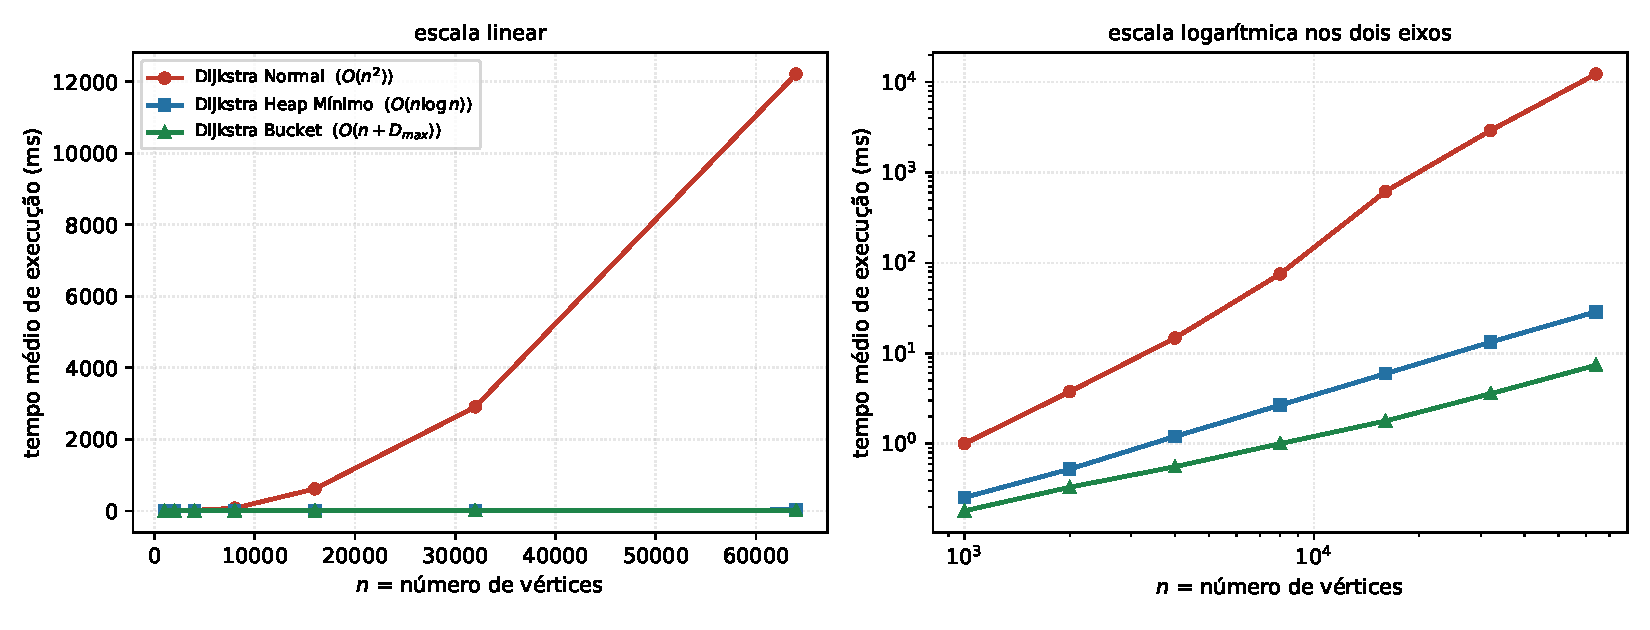
\includegraphics[width=\textwidth]{figuras/fig_tempo_vs_n.pdf}
\caption{Tempo de execução em função do tamanho da entrada $n$
(\textbf{gráfico obrigatório 1}). Em escala linear (esquerda) o crescimento
quadrático do Dijkstra Normal domina de tal forma que as outras duas curvas
ficam coladas ao eixo; a escala log--log (direita) separa as três e evidencia
inclinações diferentes.}
\label{fig:tempo}
\end{figure}

A leitura em escala linear já responde de forma bruta à pergunta central: o
Dijkstra Normal sai de $1{,}0$~ms em $n = \nMin{}$ para
$\tempoMaxNormal{}$~ms em $n = \nMax{}$, enquanto o Heap Mínimo vai a apenas
$\tempoMaxHeap{}$~ms e o Bucket a $\tempoMaxBucket{}$~ms. No maior tamanho
testado, o Heap Mínimo é cerca de \ganhoHeap{} vezes mais rápido e o Bucket
cerca de \ganhoBucket{} vezes mais rápido que a versão com varredura linear.
Vale destacar que essa diferença enorme \textbf{não vem de otimização de
código}: as três versões compartilham o gerador, a representação do grafo, o
compilador e as flags. Vem apenas da estrutura de dados escolhida para a fila
de prioridade.

\subsection{Comparação com a curva de crescimento esperada}

A Figura~\ref{fig:teoria} confronta cada série medida com a sua função de
crescimento teórica. A constante multiplicativa de cada curva teórica foi
calibrada no menor $n$ medido, ou seja, as curvas partem do mesmo ponto e o
que se compara é a \emph{forma} do crescimento, não o valor absoluto --- a
análise assintótica não prevê constantes.

\begin{figure}[H]
\centering
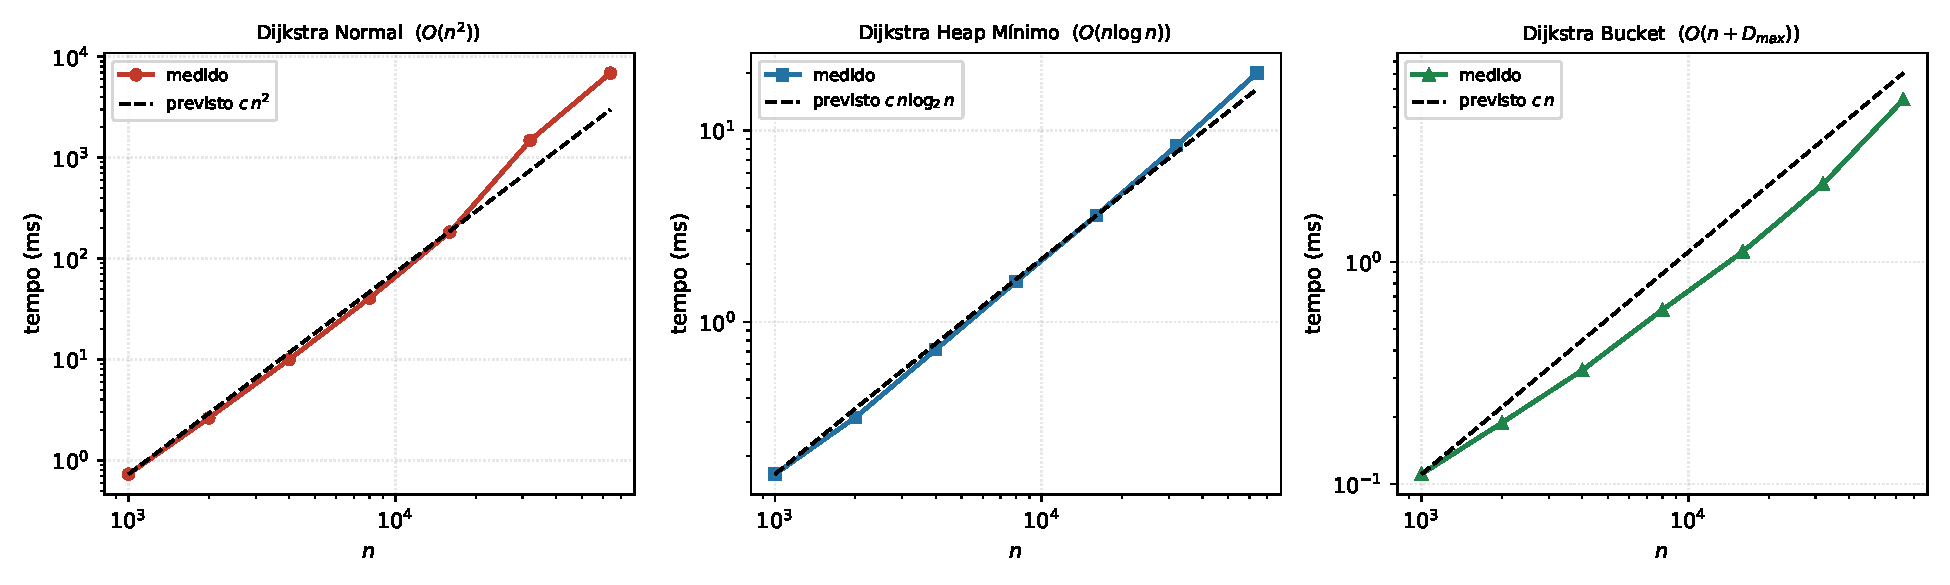
\includegraphics[width=\textwidth]{figuras/fig_teoria_vs_empirico.pdf}
\caption{Comportamento empírico \emph{versus} função de crescimento esperada
(\textbf{gráfico obrigatório 2}), em escala log--log. Linha cheia: medido;
linha tracejada: previsto, com a constante ajustada em $n = \nMin{}$.}
\label{fig:teoria}
\end{figure}

Uma forma mais sensível de comparar crescimento, que não depende de calibrar
constante alguma, é olhar a razão entre tempos de tamanhos consecutivos. Como
$n$ dobra a cada passo, essa razão deve valer aproximadamente $4$ para um
algoritmo quadrático, um pouco mais de $2$ para $n \log n$ e $2$ para um
algoritmo linear. A Tabela~\ref{tab:razoes} e a Figura~\ref{fig:razoes}
apresentam essas razões.

\begin{table}[H]
\centering
\caption{Razão de crescimento $T(2n)/T(n)$ ao dobrar o tamanho da entrada.
Valores de referência: $4$ para $O(n^2)$, pouco acima de $2$ para
$O(n\log n)$, $2$ para $O(n)$.}
\label{tab:razoes}
\small
\begin{tabular}{@{}lccc@{}}
\toprule
\textbf{Transição em $n$} & \textbf{Normal} & \textbf{Heap Mínimo} & \textbf{Bucket} \\
\midrule
\linhasRazoes
\bottomrule
\end{tabular}
\end{table}

\begin{figure}[H]
\centering
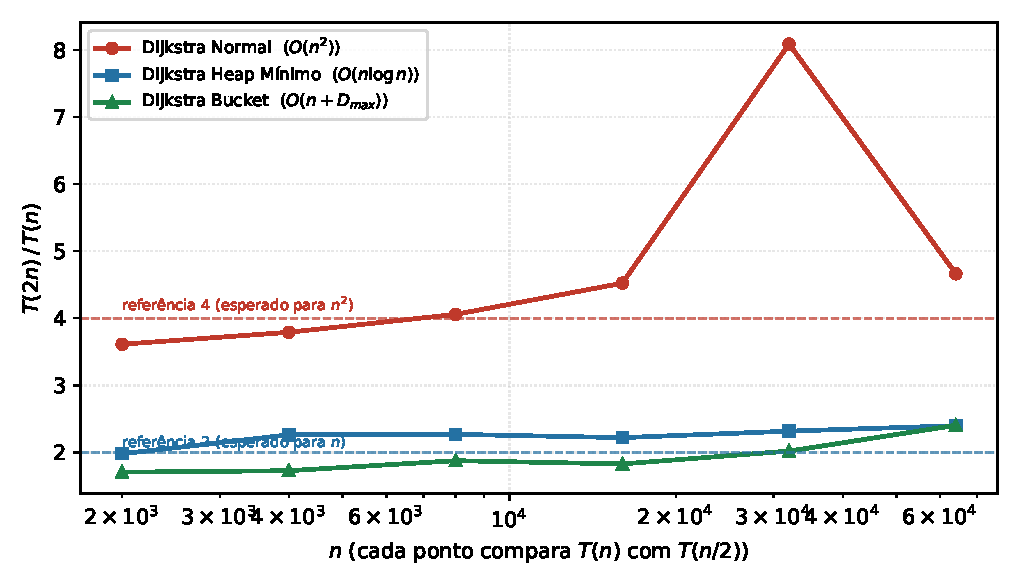
\includegraphics[width=0.72\textwidth]{figuras/fig_razoes.pdf}
\caption{Razões $T(2n)/T(n)$ medidas, com as linhas de referência $4$
(quadrático) e $2$ (linear).}
\label{fig:razoes}
\end{figure}

Complementarmente, ajustando uma reta por mínimos quadrados aos dados em
escala log--log obtemos o expoente empírico de cada variante:
$k \approx \expoenteNormal{}$ para o Normal, $k \approx \expoenteHeap{}$ para
o Heap Mínimo e $k \approx \expoenteBucket{}$ para o Bucket. Os três valores
ordenam as variantes exatamente como a teoria prevê (quadrático $>$
levemente superlinear $>$ linear), mas nenhum coincide exatamente com o
expoente ideal --- é justamente isso que a próxima seção investiga.

\subsection{Grandezas estruturais coletadas}

Para poder explicar os desvios em vez de apenas constatá-los, coletamos duas
grandezas do próprio experimento, fora da medição de tempo
(Tabela~\ref{tab:estruturais}): a maior distância final $D_{max}$, que limita
a varredura de \emph{buckets}, e o tamanho da região de memória varrida a
cada iteração do Dijkstra Normal (o vetor \texttt{dist} de 8 bytes por
vértice mais o vetor de vértices fechados de 1 byte por vértice).

\begin{table}[H]
\centering
\caption{Grandezas estruturais das instâncias (uma execução por $n$).}
\label{tab:estruturais}
\small
\begin{tabular}{@{}rrrr@{}}
\toprule
$n$ & $D_{max}$ & \emph{Buckets} vazios varridos & Memória varrida por iteração (KiB) \\
\midrule
\linhasEstruturais
\bottomrule
\end{tabular}
\end{table}

% =====================================================================
\section{Discussão: teoria \texorpdfstring{$\times$}{x} prática}
% =====================================================================

\subsection{O crescimento observado é compatível com a complexidade teórica?}

\textbf{Heap Mínimo: sim, com precisão notável.} As razões medidas ficaram
entre $2{,}06$ e $2{,}30$, contra a previsão de $2{,}20$ a $2{,}13$ deduzida
na Seção~4.2. A constante normalizada $T(n)/(n\log_2 n)$
(Tabela~\ref{tab:constantes}) permanece entre $23{,}9$ e $28{,}2$~ns enquanto
$n$ cresce $64$ vezes --- menos de $20\%$ de variação contra um aumento de
6400\% na entrada. Na Figura~\ref{fig:teoria}, a curva medida e a
curva $c\,n\log_2 n$ são praticamente indistinguíveis. Este é o caso em que
teoria e prática coincidiram melhor.

\textbf{Bucket: sim, mas o comportamento linear só aparece para $n$ grande.}
As razões começam em $1{,}82$ e $1{,}69$ --- abaixo de $2$, o que
isoladamente pareceria \emph{sublinear}, algo impossível para um algoritmo que
precisa examinar todas as $m = 4n$ arestas. A Tabela~\ref{tab:estruturais}
explica: $D_{max}$ vale $1737$ em $n = 1000$ e apenas $2615$ em
$n = 64000$, ou seja, cresce $1{,}5$ vez enquanto $n$ cresce $64$ vezes,
confirmando a previsão de que esse termo é quase independente de $n$. Em
$n = 1000$, o algoritmo varre $\approx 1938$ índices de \emph{bucket} para
processar apenas $1000$ vértices: a sobrecarga fixa \textbf{domina} o tempo.
Conforme $n$ cresce, esse custo constante se dilui, as razões sobem para
$2{,}01$ e $2{,}06$, e a constante $T(n)/n$ estabiliza em torno de
$112$--$115$~ns. Ou seja, o algoritmo é linear; o que se observava no início
era o efeito do termo aditivo $D_{max}$, exatamente como previsto.

\textbf{Normal: qualitativamente sim, quantitativamente não.} As duas
primeiras razões, $3{,}75$ e $3{,}92$, batem com o $4$ esperado. Mas as
transições seguintes dão $5{,}12$ e, sobretudo, $8{,}16$ --- o dobro do
previsto --- e só depois voltam a $4{,}73$ e $4{,}20$. O expoente empírico
global, $\expoenteNormal{}$, fica bem acima de $2$. Há aqui uma divergência
real que precisa de explicação.

\begin{table}[H]
\centering
\caption{Tempo normalizado pela função de crescimento esperada, em
nanossegundos. Um valor constante ao longo da coluna indica que a função de
crescimento escolhida descreve bem os dados.}
\label{tab:constantes}
\small
\begin{tabular}{@{}rrrr@{}}
\toprule
$n$ & $T(n)/n^2$ (Normal) & $T(n)/(n\log_2 n)$ (Heap) & $T(n)/n$ (Bucket) \\
\midrule
\linhasConstantes
\bottomrule
\end{tabular}
\end{table}

\subsection{Que fatores explicam o desvio do Dijkstra Normal?}

A causa não é o algoritmo, e sim a \textbf{hierarquia de memória}. A varredura
linear do mínimo lê, a cada uma das $n$ iterações, todo o vetor
\texttt{dist} (8 bytes por vértice) e todo o vetor de vértices fechados
(1 byte por vértice) --- cerca de $9n$ bytes. A última coluna da
Tabela~\ref{tab:estruturais} mostra o tamanho dessa região, e a comparação com
os caches da máquina (Tabela~\ref{tab:ambiente}) é reveladora:

\begin{itemize}
  \item até $n = 4000$, a região varrida ocupa no máximo $35$~KiB e cabe
        inteira na cache L1 de dados ($48$~KiB). Nessa faixa,
        $T(n)/n^2 \approx 0{,}92$--$1{,}00$~ns e as razões batem com $4$;
  \item entre $n = 8000$ e $n = 16000$ a região passa de $70$ para
        $141$~KiB e \textbf{deixa de caber na L1}, migrando para a L2. É
        exatamente aí que aparece a razão anômala de $8{,}16$: além do
        crescimento quadrático de $4\times$, cada acesso passou a custar
        mais, e os dois efeitos se multiplicaram;
  \item de $n = 16000$ em diante a região está estabilizada na L2 (que tem
        $2$~MiB, com folga até $n = 64000$) e as razões voltam a $4{,}73$ e
        $4{,}20$, com $T(n)/n^2$ estabilizando em torno de $2{,}8$--$3{,}0$~ns
        --- cerca de três vezes o valor da fase em L1.
\end{itemize}

Ou seja: o algoritmo é $\Theta(n^2)$ em número de operações, como a teoria
prevê, mas o \textbf{custo médio de cada operação triplicou} no meio do
experimento. A análise assintótica supõe custo unitário para cada acesso à
memória; máquinas reais não têm essa propriedade. O desvio observado não
refuta a teoria, ele mostra precisamente onde o modelo de custo uniforme deixa
de valer.

\subsection{Em que ponto a diferença entre os algoritmos fica evidente?}

Já em $n = 1000$ o Normal é $4$ vezes mais lento que o Heap e $5{,}5$ vezes
mais lento que o Bucket. A diferença é pequena em termos absolutos
($1$~ms contra $0{,}2$~ms) e, para uma aplicação que roda o algoritmo uma vez
sobre um grafo pequeno, escolher a estrutura ``errada'' seria irrelevante. O
quadro muda de natureza com a escala: em $n = \nMax{}$ a diferença é de
$12{,}2$ segundos contra $29$ milissegundos. É o tipo de diferença que separa
um sistema utilizável de um sistema inviável --- e é a razão prática de a
análise assintótica importar.

Entre as duas variantes eficientes, o \textbf{Bucket foi consistentemente mais
rápido que o Heap Mínimo} em toda a faixa testada, sendo cerca de
\heapSobreBucket{} vezes mais rápido em $n = \nMax{}$. Isso \emph{contraria} a
conclusão da fonte principal, que encontrou o Heap Mínimo cerca de seis vezes
mais rápido que o Bucket. A divergência é explicável e vale a pena examiná-la,
porque ilustra bem o papel das características da entrada: o custo do Bucket
carrega o termo $D_{max}$, proporcional às magnitudes das distâncias. Nas
instâncias do DIMACS usadas pela fonte, os pesos são distâncias e tempos de
viagem reais em redes de estradas, com valores muito grandes e caminhos
longos, o que torna $D_{max}$ enorme e penaliza severamente o Bucket. Nas
nossas instâncias, com pesos em $[1,1000]$ e diâmetro pequeno, $D_{max}$
ficou em torno de $2600$ e a vantagem do acesso $O(1)$ prevaleceu. Nenhum dos
dois resultados está errado: eles medem regimes de entrada diferentes, e a
lição é que a escolha da estrutura depende do perfil dos pesos, não apenas
da ordem assintótica.

\subsection{O que acontece quando \texorpdfstring{$n$}{n} aumenta muito?}

A extrapolação a partir das constantes estabilizadas é direta. Para
$n = 10^6$ com a mesma densidade, o Normal levaria aproximadamente
$3{,}0 \times (10^6)^2$~ns $\approx 50$~minutos, enquanto o Heap levaria
cerca de $28 \times 10^6 \times 20$~ns $\approx 0{,}6$~s e o Bucket
cerca de $115 \times 10^6$~ns $\approx 0{,}1$~s. Essa é a diferença
entre uma consulta interativa e um processamento em lote. A ressalva
importante é que essa extrapolação supõe que as constantes permaneçam
estáveis, e a própria Seção~6.2 mostrou que elas podem mudar quando o
conjunto de dados atravessa um nível da hierarquia de memória.

% =====================================================================
\section{Conclusão}
% =====================================================================

O experimento respondeu à pergunta central: o tempo de execução do algoritmo
de Dijkstra cresce de formas qualitativamente diferentes segundo a estrutura
de dados da fila de prioridade, e as três ordens de crescimento observadas são
compatíveis com as previsões assintóticas obtidas da análise das operações.

As principais descobertas foram:

\begin{enumerate}
  \item A variante com \textbf{Heap Mínimo} reproduziu $O(n\log n)$ com
        precisão notável: razões $T(2n)/T(n)$ entre $2{,}06$ e $2{,}30$ e
        constante normalizada praticamente estável em uma faixa de $64$ vezes
        em $n$.
  \item A variante com \textbf{Buckets} é linear, mas seu comportamento
        assintótico só se manifesta depois que $n$ supera a sobrecarga fixa
        $D_{max}$. Medir essa grandeza diretamente (que ficou entre $1737$ e
        $2615$ enquanto $n$ crescia $64$ vezes) permitiu explicar as razões
        aparentemente sublineares em vez de tratá-las como ruído.
  \item A variante \textbf{Normal} é $\Theta(n^2)$ em operações, mas seu
        tempo cresceu mais rápido que $n^2$ na faixa intermediária. A causa
        foi identificada: a região de memória varrida a cada iteração deixa
        de caber na cache L1 entre $n = 8000$ e $n = 16000$, e o custo médio
        por operação triplica. Esse é o exemplo mais didático que o trabalho
        produziu de por que ``análise assintótica descreve o crescimento, mas
        o tempo medido depende da implementação e do ambiente''.
  \item A comparação com a fonte principal levou a uma \textbf{conclusão
        oposta} quanto à disputa Heap \emph{versus} Bucket. Isso não é
        contradição: a fonte usou redes de estradas reais, com distâncias de
        magnitude muito maior, regime no qual o termo $D_{max}$ do Bucket
        pesa. A ordem assintótica não basta para escolher uma estrutura; o
        perfil da entrada importa.
\end{enumerate}

\subsection*{Limitações}

\begin{itemize}
  \item Os grafos são \textbf{aleatórios com densidade fixa} ($m = 4n$).
        Grafos reais têm estrutura (comunidades, distribuição de graus
        desigual, planaridade) que afeta tanto o diâmetro quanto a localidade
        de acesso à memória. Repetir o experimento com as instâncias do
        DIMACS usadas pela fonte permitiria comparação direta.
  \item Só a \textbf{densidade esparsa} foi testada. Em grafos densos
        ($m \approx n^2$), a vantagem do \emph{heap} diminui e o Dijkstra
        Normal volta a ser competitivo, pois seu termo $O(n^2)$ deixa de ser
        dominante.
  \item O intervalo de pesos foi fixado em $C = 1000$. Como a discussão
        mostrou, $C$ influencia diretamente o Bucket; variar $C$ mantendo $n$
        fixo seria um segundo experimento natural.
  \item As medições vêm de uma \textbf{única máquina} e de um único
        compilador. A faixa de $n$ vai até $64000$, limitada pelo tempo
        quadrático da variante Normal.
  \item Mediu-se apenas \textbf{tempo}, não consumo de memória --- que é
        justamente o ponto fraco reconhecido do \emph{heap} e dos
        \emph{buckets} frente à versão simples.
\end{itemize}

% =====================================================================
\section*{Declaração de uso de ferramentas de IA}
\addcontentsline{toc}{section}{Declaração de uso de ferramentas de IA}
% =====================================================================

Em atendimento à exigência de declarar o uso de IA em todas as etapas do
trabalho, registramos:

\begin{itemize}
  \item \textbf{Busca da fonte:} Google Acadêmico
  \item \textbf{Implementação:} os pseudocódigos das três variantes foram
        obtidos do TCC citado; a transcrição para C++, o gerador de grafos, o
        \emph{harness} de medição e a rotina de validação foram desenvolvidos
        com auxílio do assistente Claude (Anthropic), com revisão e
        verificação pelo grupo. A adaptação dos \emph{buckets} para a forma
        circular e a correção da linha~11 do pseudocódigo da fonte surgiram
        dessa revisão.
  \item \textbf{Execução do experimento:} as medições foram executadas pelo
        próprio código, sem intervenção de IA nos dados. Os valores das
        tabelas e figuras são gerados automaticamente a partir do arquivo
        \texttt{resultados/resultados\_brutos.csv} pelo script
        \texttt{codigo/gerar\_graficos.py}.
  \item \textbf{Análise e redação:} a estruturação do relatório, a redação e a
        interpretação dos resultados contaram com auxílio do mesmo assistente,
        a partir dos dados efetivamente medidos, com revisão do grupo.
  \item \textbf{Nenhum dado experimental foi gerado ou estimado por IA.}
\end{itemize}

% =====================================================================
\addcontentsline{toc}{section}{Referências}
% =====================================================================

\begin{thebibliography}{9}
\small

\bibitem{cormen}
CORMEN, T. H.; LEISERSON, C. E.; RIVEST, R. L.; STEIN, C.
\textbf{Algoritmos: Teoria e Prática}. 3. ed. Rio de Janeiro: Elsevier, 2009.

\bibitem{dial}
DIAL, R. B. Algorithm 360: Shortest-path forest with topological ordering.
\textbf{Communications of the ACM}, v. 12, n. 11, p. 632--633, 1969.

\bibitem{dijkstra}
DIJKSTRA, E. W. A note on two problems in connexion with graphs.
\textbf{Numerische Mathematik}, v. 1, p. 269--271, 1959.

\bibitem{dimacs}
DIMACS. \textbf{9th DIMACS Implementation Challenge --- Shortest Paths}.
Disponível em:
\url{https://www.diag.uniroma1.it/challenge9/download.shtml}.
Acesso em: 08/09/2026.

\bibitem{tcc}
RODRIGUES, G. C. S. \textbf{Análise de desempenho do algoritmo de Dijkstra com
diferentes estruturas de dados}. 2023. Trabalho de Conclusão de Curso
(Bacharelado em Ciência da Computação) --- Universidade Federal do Espírito
Santo, Alegre, 2023. Código-fonte disponível em:
\url{https://github.com/guiconrado/Djkstra}.

\bibitem{sedgewick}
SEDGEWICK, R.; WAYNE, K. \textbf{Algorithms}. 4. ed. Boston: Addison-Wesley
Professional, 2011.

\bibitem{tarjan}
TARJAN, R. E. \textbf{Data Structures and Network Algorithms}. Philadelphia:
Society for Industrial and Applied Mathematics, 1983.

\end{thebibliography}

% =====================================================================
\section{Repositório do trabalho no GitHub: }
% =====================================================================

\quad{https://github.com/marcuslsza/analise-djikstra-edb2}

\end{document}